\documentclass[aspectratio=169]{beamer}

% Theme and color scheme
\usetheme{Madrid}
\usecolortheme{seahorse}

% Packages
\usepackage[utf8]{inputenc}
\usepackage{graphicx}
\usepackage{amsmath}
\usepackage{amssymb}
\usepackage{tikz}
\usepackage{booktabs}
\usepackage{subcaption}
\usepackage{xcolor}

% Custom colors
\definecolor{rayblue}{RGB}{0, 122, 204}
\definecolor{awsorange}{RGB}{255, 153, 0}
\definecolor{hpcgreen}{RGB}{0, 153, 76}

% Title information
\title[Optimizing Vector Algorithm Processing]{Optimizing Vector Algorithm Processing through the integration of Ray IO and HPC in the Cloud}
\author{Tiago de Souza de Oliveira}
\institute[University]{
    Master's Thesis Defense \\
    Computer Science Department
}
\date{\today}

% Footer information
\setbeamertemplate{footline}[frame number]

\begin{document}

% Title slide
\frame{\titlepage}

% Slide 1: The New Frontier
\begin{frame}{The New Frontier: Scaling Scientific Workflow with ETL and AI Workloads}
    \begin{columns}
        \begin{column}{0.6\textwidth}
            \textbf{Context \& Motivation:}
            \begin{itemize}
                \item \textbf{Large-scale AI} (NLP, Computer Vision) and \textbf{scientific domains} (drug discovery, genomics, CFD) rely on processing vast raw datasets
                \item Transform raw knowledge into \textcolor{rayblue}{\textbf{dense numeric arrays (embeddings)}} for downstream algorithms
                \item \textbf{Traditional HPC limitations on pre-processing:} massive capital investment, long procurement cycles, struggles with data-intensive I/O
                \item Map-Reduce and Apache Spark often \textbf{falls short at petabyte-scale processing and lack efficient capabilities for distributed training AI models}
            \end{itemize}
        \end{column}
        \begin{column}{0.4\textwidth}
            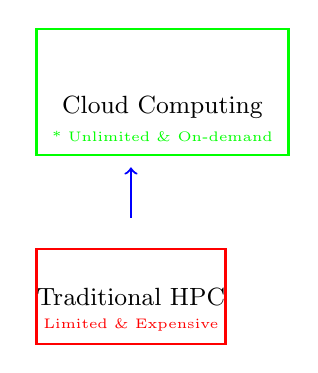
\begin{tikzpicture}[scale=0.8]
                % Traditional HPC box
                \draw[thick, red] (0,0) rectangle (3,1.5);
                \node at (1.5,0.75) {\small Traditional HPC};
                \node[red] at (1.5,0.3) {\tiny Limited \& Expensive};
                
                % Arrow
                \draw[->, thick, blue] (1.5, 2) -- (1.5, 2.8);
                
                % Cloud box
                \draw[thick, green] (0,3) rectangle (4,5);
                \node at (2,3.75) {\small Cloud Computing};
                \node[green] at (2,3.3)  {\tiny * Unlimited \& On-demand};
            \end{tikzpicture}
        \end{column}
    \end{columns}
    
    \vspace{0.3cm}
    \begin{alertblock}{The Opportunity}
        Cloud computing offers \textbf{unlimited, on-demand capacity} with up to \textcolor{awsorange}{\textbf{90\% cost savings}} through EC2 Spot Instances and Infrastructure-as-Code
    \end{alertblock}
\end{frame}

\begin{frame}{A Two-Phased Cloud-Native Architecture for Optimization}
    \begin{center}
        \includegraphics[width=0.9\textwidth,height=0.6\textheight,keepaspectratio]{TFM-MindMap.drawio.png}
    \end{center}
    
    \vspace{0.3cm}
    \begin{block}{Key Integration}
        \textbf{Unified storage layer} bridges Phase 1 outputs with Phase 2 inputs, enabling seamless data flow and high-throughput access
    \end{block}
    
    \vspace{0.2cm}
    \textbf{Example:} Metagenomics pipeline - FASTQ reads → k-mer embeddings → organism clustering
\end{frame}


% Slide 2: Two-Phased Architecture
\begin{frame}{A Two-Phased Cloud-Native Architecture for Optimization}
    \begin{center}
        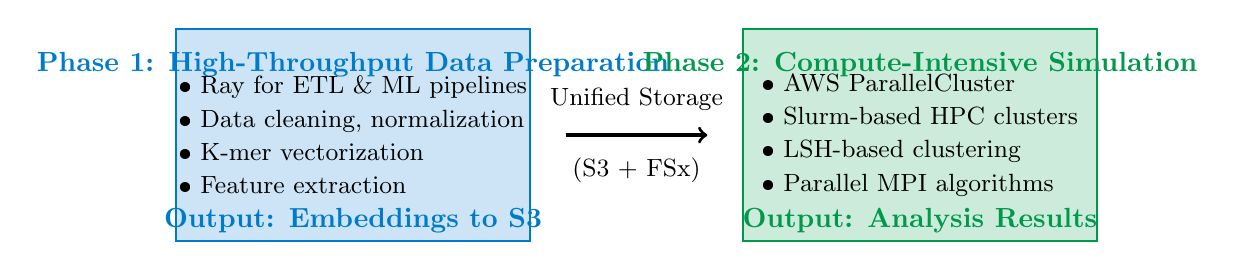
\begin{tikzpicture}[scale=0.9]
            % Phase 1 box
            \draw[thick, rayblue, fill=rayblue!20] (0,0) rectangle (5,3);
            \node[rayblue, font=\bfseries] at (2.5,2.5) {Phase 1: High-Throughput Data Preparation};
            \node[align=left] at (2.5,1.5) {
                \small • Ray for ETL \& ML pipelines \\
                \small • Data cleaning, normalization \\
                \small • K-mer vectorization \\
                \small • Feature extraction
            };
            \node[rayblue] at (2.5,0.3) {\textbf{Output: Embeddings to S3}};
            
            % Arrow
            \draw[->, very thick, black] (5.5, 1.5) -- (7.5, 1.5);
            \node at (6.5, 2) {\small Unified Storage};
            \node at (6.5, 1) {\small (S3 + FSx)};
            
            % Phase 2 box
            \draw[thick, hpcgreen, fill=hpcgreen!20] (8,0) rectangle (13,3);
            \node[hpcgreen, font=\bfseries] at (10.5,2.5) {Phase 2: Compute-Intensive Simulation};
            \node[align=left] at (10.5,1.5) {
                \small • AWS ParallelCluster \\
                \small • Slurm-based HPC clusters \\
                \small • LSH-based clustering \\
                \small • Parallel MPI algorithms
            };
            \node[hpcgreen] at (10.5,0.3) {\textbf{Output: Analysis Results}};
        \end{tikzpicture}
    \end{center}
    
    \vspace{0.3cm}
    \begin{block}{Key Integration}
        \textbf{Unified storage layer} bridges Phase 1 outputs with Phase 2 inputs, enabling seamless data flow and high-throughput access
    \end{block}
    
    \vspace{0.2cm}
    \textbf{Example:} Metagenomics pipeline - FASTQ reads → k-mer embeddings → organism clustering
\end{frame}

% Slide 3: Phase 1 Deep Dive
\begin{frame}{Phase 1 Deep Dive: Ray for Scalable Data Preprocessing}
    \begin{columns}
        \begin{column}{0.5\textwidth}
            \textbf{Ray's Role in Data Preparation:}
            \begin{itemize}
                \item \textbf{Data Ingestion:} Raw FASTQ reads processing
                \item \textbf{K-mer Embeddings:} Using \textcolor{rayblue}{\textbf{DNABERT-2-117M}} for fixed-length numeric vectors
                \item \textbf{Parallel Processing:} Lightweight tasks across CPUs/GPUs
                \item \textbf{Output:} Parquet shards to Amazon S3
            \end{itemize}
        \end{column}
        \begin{column}{0.5\textwidth}
            \textbf{Performance \& Efficiency:}
            \begin{table}[h]
                \centering
                \small
                \begin{tabular}{lc}
                    \toprule
                    \textbf{Metric} & \textbf{Result} \\
                    \midrule
                    Scaling (1→2 GPUs) & 2× throughput \\
                    Processing rate & ~22 MB/s \\
                    Node startup time & ~90s \\
                    Spot Instance savings & \textcolor{green}{\textbf{65\%}} \\
                    Cost per GB & \textcolor{green}{\textbf{\$0.12}} \\
                    \bottomrule
                \end{tabular}
            \end{table}
        \end{column}
    \end{columns}
    
    \vspace{0.3cm}
    \begin{alertblock}{Key Achievement}
        \textbf{Near-linear scaling} with Ray autoscaler dynamically managing cluster size and achieving \textcolor{green}{\textbf{65\% cost reduction}} through Spot Instances
    \end{alertblock}
\end{frame}

% Slide 4: Phase 2 Deep Dive
\begin{frame}{Phase 2 Deep Dive: HPC for Compute-Intensive Simulation \& Overall Impact}
    \begin{columns}
        \begin{column}{0.6\textwidth}
            \textbf{HPC Simulation with AWS ParallelCluster:}
            \begin{itemize}
                \item \textbf{Embedding Consumption:} Direct access from FSx/S3
                \item \textbf{Specialized Compute:} P4d instances with \textcolor{awsorange}{\textbf{NVIDIA A100 GPUs}}
                \item \textbf{Low-latency Communication:} Elastic Fabric Adapter (EFA) for MPI
                \item \textbf{Clustering Algorithms:} Parallel LSH and k-means for organism grouping
            \end{itemize}
        \end{column}
        \begin{column}{0.4\textwidth}
            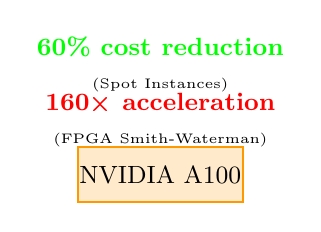
\begin{tikzpicture}[scale=0.7]
                % GPU representation
                \draw[thick, awsorange, fill=awsorange!20] (0,0) rectangle (3,1);
                \node at (1.5,0.5) {\small NVIDIA A100};
                
                % Performance metrics
                \node[align=center] at (1.5,1.5) {\small \textcolor{red}{\textbf{160× acceleration}} \\ \tiny (FPGA Smith-Waterman)};
                
                % Cost savings
                \node[align=center] at (1.5,2.5) {\small \textcolor{green}{\textbf{60\% cost reduction}} \\ \tiny (Spot Instances)};
            \end{tikzpicture}
        \end{column}
    \end{columns}
    
    \vspace{0.3cm}
    \begin{block}{Synergistic Performance \& Benefits}
        \begin{itemize}
            \item \textbf{Hardware Acceleration:} FPGAs achieve \textcolor{red}{\textbf{160-fold acceleration}} for Smith-Waterman algorithms
            \item \textbf{Extreme-scale Processing:} GPU-enabled protein similarity searches across hundreds of millions of proteins in hours vs. weeks
            \item \textbf{Cost Optimization:} \textcolor{green}{\textbf{Over 60\% infrastructure cost reduction}} through Spot Instances
            \item \textbf{Developer Agility:} Unified cloud-agnostic control plane streamlines complex pipelines
        \end{itemize}
    \end{block}
\end{frame}

% Slide 5: Conclusions
\begin{frame}{Conclusions}
    \begin{columns}
        \begin{column}{0.6\textwidth}
            \textbf{Key Conclusions:}
            \begin{itemize}
                \item Two-phase architecture delivers \textbf{significant gains} in scalability, elasticity, performance, and cost-efficiency
                \item \textcolor{rayblue}{\textbf{GPU-accelerated Ray clusters scale nearly linearly}} for DNA embedding extraction
                \item Automated lifecycle management and Spot Instances ensure \textcolor{green}{\textbf{optimized resource utilization}}
                \item Successfully \textbf{decouples feature engineering from raw simulation workloads}
            \end{itemize}
        \end{column}
        \begin{column}{0.4\textwidth}
            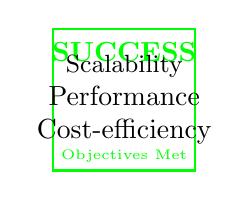
\begin{tikzpicture}[scale=0.6]
                % Success metrics visualization
                \draw[thick, green] (0,0) -- (0,3) -- (3,3) -- (3,0) -- cycle;
                \node[green, font=\bfseries] at (1.5,2.5) {SUCCESS};
                \node[align=center] at (1.5,1.5) {\small Scalability \\ Performance \\ Cost-efficiency};
                \node[green] at (1.5,0.3) {\tiny Objectives Met};
            \end{tikzpicture}
        \end{column}
    \end{columns}
    
    \vspace{0.3cm}
    \begin{block}{Future Work \& Research Avenues}
        \begin{itemize}
            \item \textbf{FPGA Workloads:} Explore AWS F1 instances using Xilinx Vitis for \textcolor{red}{\textbf{orders-of-magnitude speedups}}
            \item \textbf{Apple M-Series SoCs:} Investigate Ray's affinity scheduling on macOS for edge prototyping
            \item \textbf{Managed ETL \& Conversational DevOps:} Balance AWS Glue with deep AI tasks, integrate \textcolor{rayblue}{\textbf{domain-aware LLM agents}} for automated CloudFormation/CDK generation
        \end{itemize}
    \end{block}
\end{frame}

% Slide 6: Future Directions
\begin{frame}{Future Directions}
    \begin{columns}
        \begin{column}{0.6\textwidth}
            \textbf{Key Emerging Capabilities:}
            \begin{itemize}
                \item Two-phase architecture delivers \textbf{significant gains} in scalability, elasticity, performance, and cost-efficiency
                \item \textcolor{rayblue}{\textbf{GPU-accelerated Ray clusters scale nearly linearly}} for DNA embedding extraction
                \item Automated lifecycle management and Spot Instances ensure...
                \item Successfully \textbf{decouples feature ...}
            \end{itemize}
        \end{column}
        \begin{column}{0.4\textwidth}
            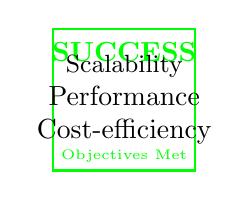
\begin{tikzpicture}[scale=0.6]
                % Success metrics visualization
                \draw[thick, green] (0,0) -- (0,3) -- (3,3) -- (3,0) -- cycle;
                \node[green, font=\bfseries] at (1.5,2.5) {SUCCESS};
                \node[align=center] at (1.5,1.5) {\small Scalability \\ Performance \\ Cost-efficiency};
                \node[green] at (1.5,0.3) {\tiny Objectives Met};
            \end{tikzpicture}
        \end{column}
    \end{columns}
    
    \vspace{0.3cm}
    \begin{block}{Future Work \& Research Avenues}
        \begin{itemize}
            \item \textbf{FPGA Workloads:} Explore AWS F1 instances using Xilinx Vitis for \textcolor{red}{\textbf{orders-of-magnitude speedups}}
            \item \textbf{Apple M-Series SoCs:} Ray's  macOS  edge 
            \item \textbf{Managed ETL \& Conversational DevOps:} agentic AI integrate \textcolor{rayblue}{\textbf{domain-aware LLM agents}} for automated CloudFormation/CDK generation
        \end{itemize}
    \end{block}
\end{frame}

% Thank you slide
\begin{frame}[plain]
    \begin{center}
        \Huge Thank You!
        
        \vspace{1cm}
        \Large Questions?
        
        \vspace{0.8cm}
        \normalsize
        \textbf{Optimizing Vector Algorithm Processing through the integration of Ray IO and HPC in the Cloud}
        
        \vspace{0.5cm}
        Tiago de Souza de Oliveira \\
        \texttt{tiago.souza@rai.usc.es, tiagoooliveira@qmind-lab.com}
    \end{center}
\end{frame}

\end{document}